\documentclass[
  11pt,
  letterpaper,
   addpoints,
   %answers
  ]{exam}

\usepackage{../exercise-preamble}
\usepackage{float}
% TikZ libraries needed for `right=.. of ..` and coordinate math
\usetikzlibrary{positioning,calc,arrows,arrows.meta}
% Alias de seguridad por si se escribe 'ikzstyle' por error
\let\ikzstyle\tikzstyle

\begin{document}

\noindent
\begin{minipage}{0.47\textwidth}

\includegraphics[width=\textwidth]{../fcfm_die}
\end{minipage}
\begin{minipage}{0.53\textwidth}
\begin{center} 
\large\textbf{Análisis de señales} (EL3203-2) \\
\large\textbf{Clase auxiliar 2} \\
\normalsize Prof.~Jorge Silva.\\
\normalsize Prof.~Aux.~Erik Sáez
\end{center}
\end{minipage}

\vspace{0.5cm}
\noindent
\vspace{.85cm}

\begin{questions}
    %%%%%%%%%%%%%%%%%%%%%%%%%%%
\question Sean los siguientes sistemas a tiempo discreto:

\begin{enumerate}
\item Determine si los siguientes sistemas a tiempo discreto son lineales y/o invariantes en el tiempo:
\begin{itemize}
\item $y[n] = nx[n]$
\item $y[n] = e^{x[n]}$
\item $y[n] = \sum_{j=1}^{M} a_j \cdot x[n-j] + B$
\end{itemize}

\item Para el sistema a tiempo discreto T definido por la relación entrada-salida $y[n] = n\,x[n]$, bosqueje por separado $T_k\big(T(x[n])\big)$ y $T\big(T_k(x[n])\big)$ para $k = 2$ y compare con los resultados obtenidos en la parte a. Para el bosquejo considere la señal:
\begin{equation}
x[n] = \begin{cases}
1 & 0 \leq n \leq 2 \\
0 & \text{en otro caso}
\end{cases}
\end{equation}
\end{enumerate}
%--------------------------------
\begin{solution}
  \subsection*{Resolución 1.1}
Se busca determinar si los sistemas corresponden a sistemas lineales y/o invariantes en el tiempo, dado que cuando cumplen ambas condiciones en simultáneo podemos decir que el sistema será LTI, lo que tiene varias ventajas, como por ejemplo:
\begin{itemize}
  \item Simplificación del análisis y diseño de sistemas.
  \item Posibilidad de utilizar la transformada de Fourier para analizar la respuesta en frecuencia.
  \item Aplicación de técnicas de convolución para determinar la salida del sistema.
\end{itemize}
Estas dos condiciones vienen caracterizadas por lo siguiente:
\begin{itemize}
  \item \textbf{Linealidad:} Un sistema es lineal si cumple con el principio de superposición, es decir, para cualesquiera dos señales de entrada \(x_1[n]\) y \(x_2[n]\), y cualesquiera dos constantes escalares \(\alpha\) y \(\beta\), la respuesta del sistema a la combinación lineal de las entradas debe ser igual a la combinación lineal de las respuestas individuales; matemáticamente,
  \begin{equation}
    T(\alpha x_1[n] + \beta x_2[n]) = \alpha T(x_1[n]) + \beta T(x_2[n])
  \end{equation}
  \item \textbf{Invariancia temporal:} Un sistema es invariante en el tiempo si un desplazamiento en la entrada produce un desplazamiento idéntico en la salida, sin cambiar la forma de la señal.
  \begin{equation}
    T_k(T(x[n])) = T(T_k(x[n]))
  \end{equation}
\end{itemize}
Luego analizando cada caso tenemos que:

  \paragraph{(i) $T(x[n])= n \, x[n] = y[n]$}
\begin{itemize}
  \item \textbf{Linealidad:}
  \begin{align}
  T(\alpha x_1[n] + \beta x_2[n]) 
    &= n(\alpha x_1[n] + \beta x_2[n]) \\
    &= \alpha \, n x_1[n] + \beta \, n x_2[n] \\
    &= \alpha T(x_1[n]) + \beta T(x_2[n])
  \end{align}
  Por lo tanto, el sistema es \textbf{lineal}.
  \item \textbf{Invarianza temporal:}
  Tenemos que el sistema deberá cumplir que $T_{k}(T(x[n])) = T(T_{k}(x[n]))$, donde tenemos que:
  \begin{align}
  T(x[n]) &= n x[n] \\
  T_k(n x[n]) &= (n-k)x[n-k] \\
  \end{align}
  Por otro lado
  \begin{align}
  T_k(x[n]) &= x[n-k]\\
  T(x[n-k]) &= n \, x[n-k]
  \end{align}
  Como se tiene que:
  \begin{equation}
  (n-k)x[n-k] \neq n x[n-k],
  \end{equation}
  el sistema \textbf{no es invariante en el tiempo}.
\end{itemize}

  % --- Caso (ii) ---
  \paragraph{(ii) $T(x[n]) = e^{x[n]} = y[n]$}
\begin{itemize}
  \item \textbf{Linealidad:}
  \begin{align}
  T(\alpha x_1[n] + \beta x_2[n]) &= e^{\alpha x_1[n] + \beta x_2[n]} \\
  &\neq \alpha e^{x_1[n]} + \beta e^{x_2[n]} \\
  &= \alpha T(x_1[n]) + \beta T(x_2[n])
  \end{align}
  Por lo tanto, el sistema es \textbf{no lineal}.
  \item \textbf{Invarianza temporal:}
  Tenemos que el sistema deberá cumplir que $T_{k}(T(x[n])) = T(T_{k}(x[n]))$, donde tenemos que:
  \begin{align}
  T(x[n]) &= e^{x[n]} \\
  T_k(e^{x[n]}) &= e^{x[n-k]} \\
  \end{align}
  Por otro lado
  \begin{align}
  T_k(x[n]) &= x[n-k]\\
  T(x[n-k]) &= e^{x[n-k]}
  \end{align}
  Como
  \begin{equation}
  T_k(T(x[n])) = T(T_k(x[n])),
  \end{equation}
  el sistema es \textbf{invariante en el tiempo}.
\end{itemize}

  % --- Caso (iii) ---
  \paragraph{(iii) $T(x[n]) = \sum_{j=1}^{M} a_j \, x[n-j] + B = y[n]$}
\begin{itemize}
  \item \textbf{Linealidad:}
  \begin{align}
  T(\alpha x_1[n] + \beta x_2[n]) 
    &= \sum_{j=1}^{M} a_j \big( \alpha x_1[n-j] + \beta x_2[n-j] \big) + B \\
    &= \alpha \sum_{j=1}^{M} a_j x_1[n-j] + \beta \sum_{j=1}^{M} a_j x_2[n-j] + B
  \end{align}
  Mientras que:
  \begin{align}
  \alpha T(x_1[n]) + \beta T(x_2[n]) 
    &= \alpha \Big( \sum_{j=1}^{M} a_j x_1[n-j] + B \Big) 
     + \beta \Big( \sum_{j=1}^{M} a_j x_2[n-j] + B \Big) \\
    &= \alpha \sum_{j=1}^{M} a_j x_1[n-j] + \beta \sum_{j=1}^{M} a_j x_2[n-j] + (\alpha+\beta)B
  \end{align}
  Como aparece un término adicional $(\alpha+\beta)B \neq B$, el sistema es \textbf{no lineal}.
  \item \textbf{Invarianza temporal:}
  Tenemos que el sistema deberá cumplir que $T_{k}(T(x[n])) = T(T_{k}(x[n]))$, donde tenemos que:
  \begin{align}
  T(x[n]) &= \sum_{j=1}^{M} a_j x[n-j] + B  \\
  T_k(\sum_{j=1}^{M} a_j x[n-j] + B ) &= \sum_{j=1}^{M} a_j x[(n-k)-j] + B \\
  \end{align}
  Por otro lado
  \begin{align}
  T_k(x[n]) &= x[n-k]\\
  T(x[n-k]) &= \sum_{j=1}^{M} a_j x[n-k-j] + B
  \end{align}
  Como
  \begin{equation}
  T_k(T(x[n])) = T(T_k(x[n])),
  \end{equation}
  el sistema es \textbf{invariante en el tiempo}.
\end{itemize}
\subsection*{Resolución 1.2}

Para verificar si el sistema $T(x[n]) = n\,x[n]$ es invariante en el tiempo, se comparan las composiciones $T_k(T(x[n]))$ y $T(T_k(x[n]))$ para $k = 2$, donde $T_k$ representa un desplazamiento de dos muestras hacia la derecha. La señal de prueba es:
\begin{equation}
x[n] = \begin{cases}
1 & 0 \leq n \leq 2 \\
0 & \text{en otro caso}
\end{cases}
\end{equation}
Gráficamente, $x[n]$ se ve así:
\begin{figure}[H]
  \centering
  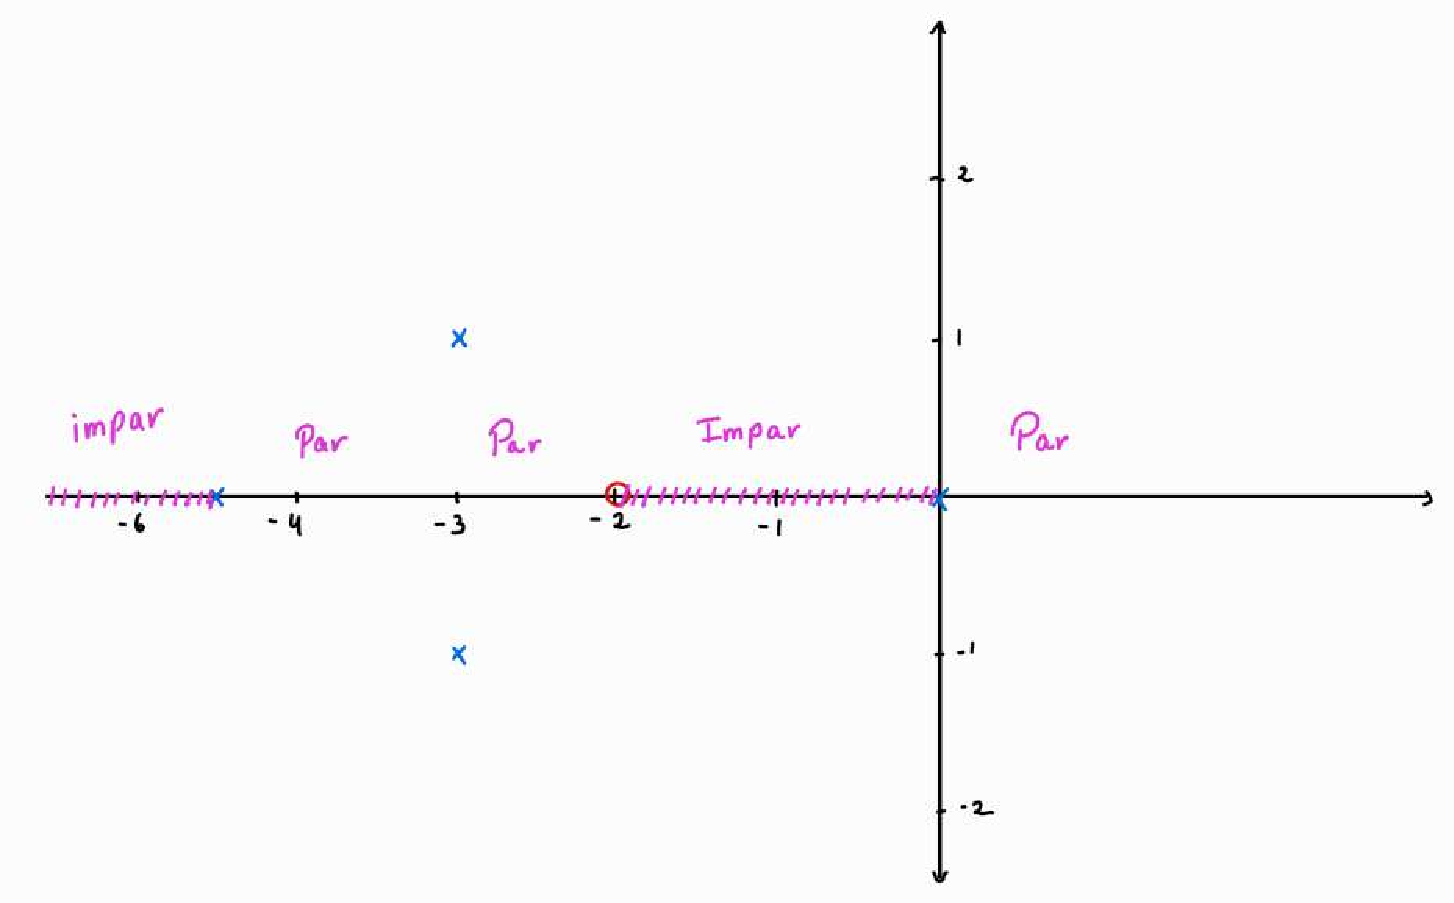
\includegraphics[width=0.5\textwidth]{Auxiliar_2_1}
  \caption{Señal $x[n] = 1$ para $0\le n\le 2$ y 0 en otro caso.}
\end{figure}

La figura siguiente resume las operaciones aplicadas sobre $x[n]$ y sus resultados intermedios/finales:

\begin{figure}[H]
  \centering
  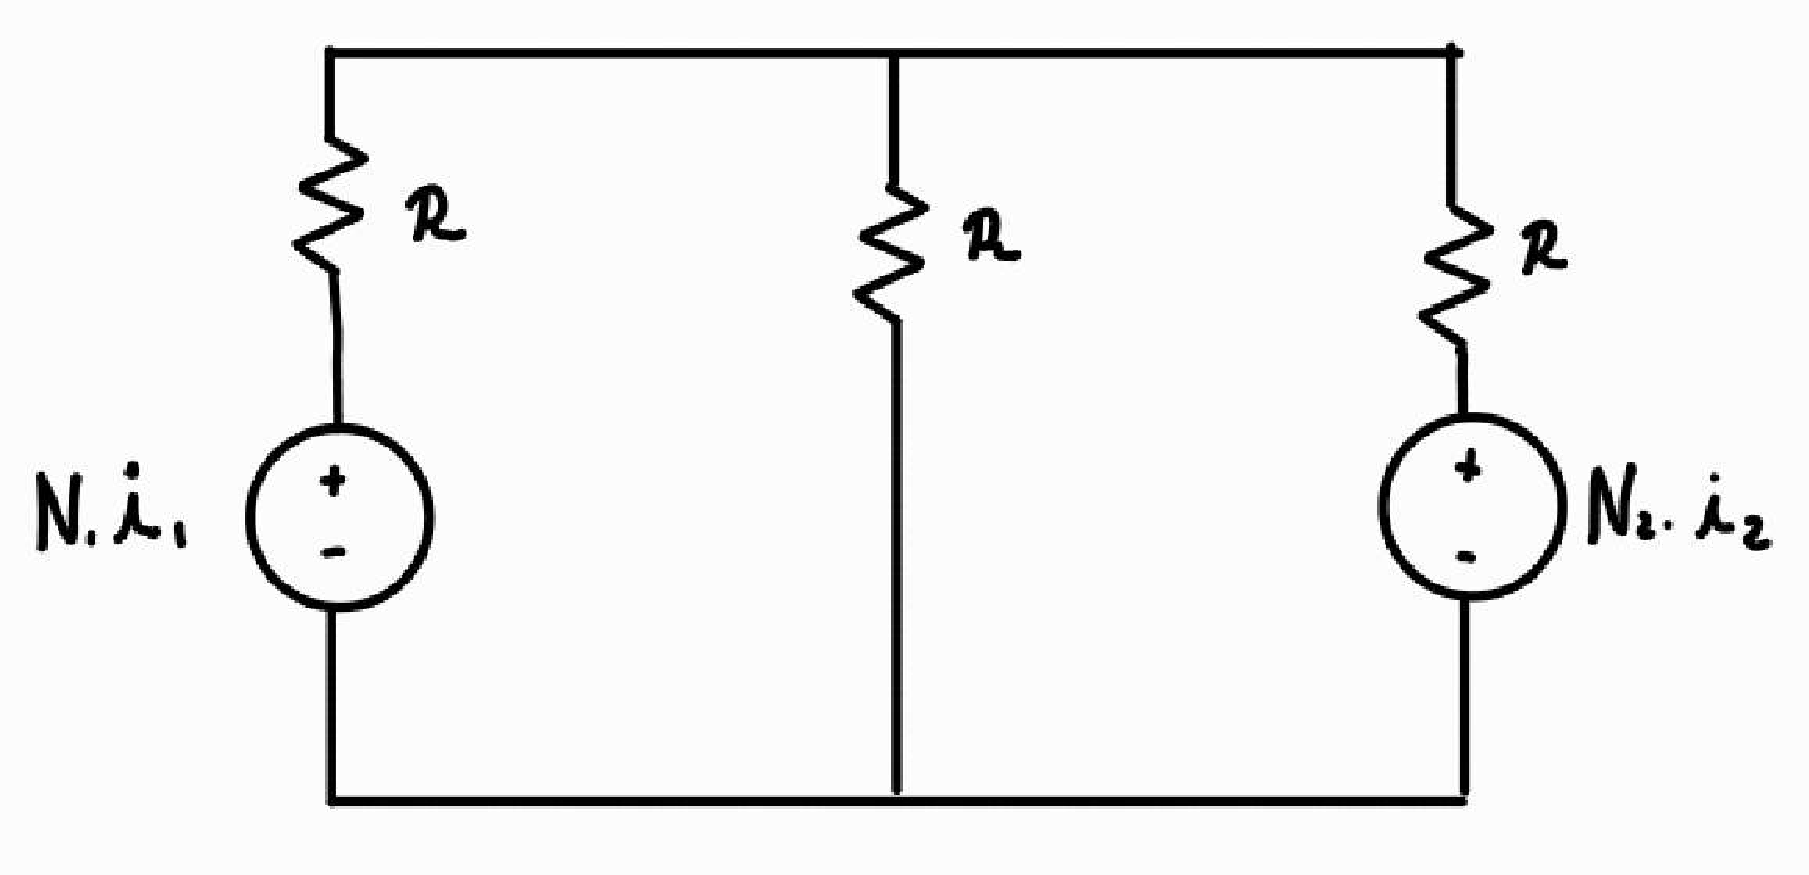
\includegraphics[width=0.9\textwidth]{Auxiliar_2_2}
  \caption{Comparación de operaciones. Arriba izq.: $T_2(x)[n]=x[n-2]$. Arriba der.: $T(T_2(x))[n]=n\,x[n-2]$. Abajo izq.: $T(x)[n]=n\,x[n]$. Abajo der.: $T_2(T(x))[n]=(n-2)\,x[n-2]$.}
\end{figure}

En relación con la figura anterior, notamos que $\,T_2(T(x[n])) \neq T(T_2(x[n]))\,$; el sistema $y[n]=n\,x[n]$ \textbf{no es invariante en el tiempo}. La diferencia surge porque el factor de escalamiento depende de $n$; al desplazar la señal, cambia el valor del multiplicador temporal.
\end{solution}
%%%%%%%%%%%%%%%%%%%%%%%%%%%
\question Escriba el siguiente sistema, bosqueje la salida del sistema si a la entrada hay un impulso de magnitud 1 centrado en 0 y clasifique esa señal de salida en cuanto a su energía y si corresponde, su potencia.
\begin{figure}[H]
  \centering
  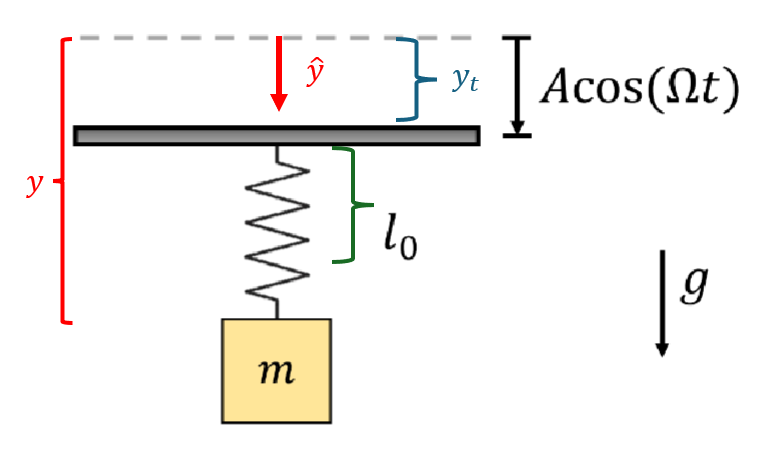
\includegraphics[width=0.8\textwidth]{Auxiliar_2_4}
\end{figure}
\begin{solution}
\subsection*{Resolución 2.1}
Recordemos que los símbolos $z^{-n}$ corresponden a retardos de $n$ muestras en el dominio temporal. Además, el bloque suma hace referencia a sumar todas las entradas que recibe. Por lo tanto, la ecuación que representa el sistema es la siguiente:
\begin{equation}
y[n] = A\,[\,x[n] + x[n-1] + x[n-2]\,] + y[n-1].
\end{equation}
Considerando que el sistema estaba en reposo, la respuesta ante la entrada $x[n] = \delta[n]$ es:

\[
\begin{array}{|c|c|c|}
\hline
n & x[n] & y[n] \\
\hline
-2 & 0 & 0 \\
-1 & 0 & 0 \\
0 & 1 & A \\
1 & 0 & 2A \\
2 & 0 & 3A \\
3 & 0 & 3A \\
4 & 0 & 3A \\
\vdots & \vdots & \vdots \\
\hline
\end{array}
\]
Si se bosqueja la salida, se obtiene una secuencia causal que comienza en $n=0$ con amplitud $A$, 
en $n=1$ alcanza $2A$, y desde $n=2$ en adelante permanece constante en $3A$, es decir:
\begin{equation}
y[n] = 
\begin{cases}
A, & n=0, \\
2A, & n=1, \\
3A, & n \geq 2, \\
0, & n<0.
\end{cases}
\end{equation}
Se bosqueja a continuación:
\begin{figure}[H]
  \centering
  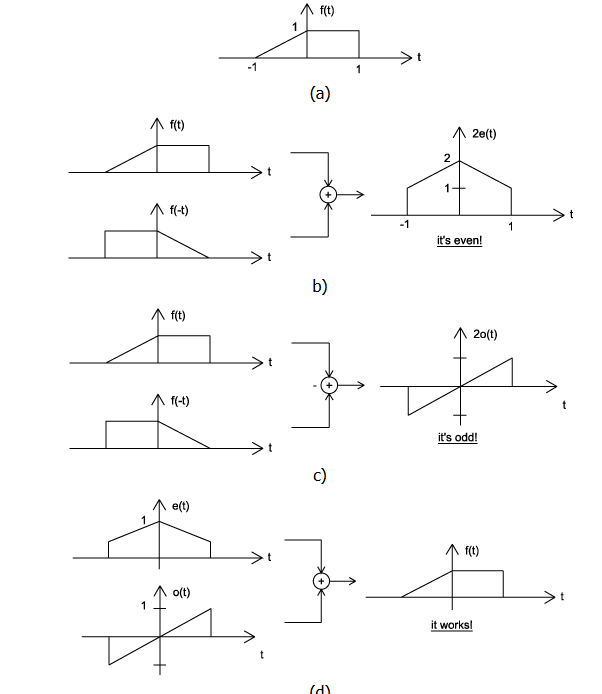
\includegraphics[width=0.5\textwidth]{Auxiliar_2_3}
  \caption{Respuesta del sistema a la entrada $\delta[n]$.}
\end{figure}
Luego, se busca analizar la energía y la potencia; recordemos que sus definiciones son:
\begin{itemize}
  \item \textbf{Energía:} La energía de una señal $y(n)$ se define como la suma de los cuadrados de sus valores absolutos a lo largo de todo el tiempo:
\begin{equation}
E = \sum_{n=-\infty}^{\infty} |y(n)|^2.
\end{equation}
\item \textbf{Potencia:} La potencia de una señal $y(n)$ se define como el valor promedio de la energía por unidad de tiempo:
\begin{equation}
P = \lim_{N \to \infty} \frac{1}{2N+1} \sum_{n=-N}^{N} |y(n)|^2.
\end{equation}
\end{itemize}
Se dice que una señal es de energía cuando
\begin{equation}
E = \sum_{n=-\infty}^{\infty} |y(n)|^2 < \infty,
\end{equation}
y una señal es de potencia cuando
\begin{equation}
0 < P = \lim_{N \to \infty} \frac{1}{2N+1} \sum_{n=-N}^{N} |y(n)|^2 < \infty.
\end{equation}
Luego para nuestro caso en particular tenemos lo siguiente:
\begin{itemize}
\item \textbf{Energía:} 
\begin{align}
E &= \sum_{n=-\infty}^{\infty} |y(n)|^2 \\
  &= A^2 + (2A)^2 + \sum_{n=2}^{\infty} (3A)^2.
\end{align}

La última suma es infinita, por lo tanto:
\begin{equation}
E \to \infty \quad \Rightarrow \quad \text{la energía diverge, es decir, la señal no es de energía.}
\end{equation}

\item \textbf{Potencia:}  
\begin{align}
P &= \lim_{N\to\infty} \frac{1}{2N+1} \sum_{n=-N}^{N} |y(n)|^2 \\
  &= \lim_{N\to\infty} \frac{1}{2N+1} 
     \left[ A^2 + (2A)^2 + \sum_{n=2}^{N} (3A)^2 \right] \\
  &= \lim_{N\to\infty} \frac{(N-1)(3A)^2}{2N+1} \\
  &= \frac{9A^2}{2}.
\end{align}
\end{itemize}

Por lo tanto, la señal de salida es una \textbf{señal de potencia} con 
\begin{equation}
P = \frac{9A^2}{2}.
\end{equation}
\end{solution}
%---------------------------------------
\question Considere el sistema mostrado en la figura, donde \(h[n]=a^n u[n]\) con \(-1<a<1\). Determine la respuesta del sistema bajo la excitación
\[x[n]=u[n+5]-u[n-10].\]

\begin{figure}[H]
  \centering
  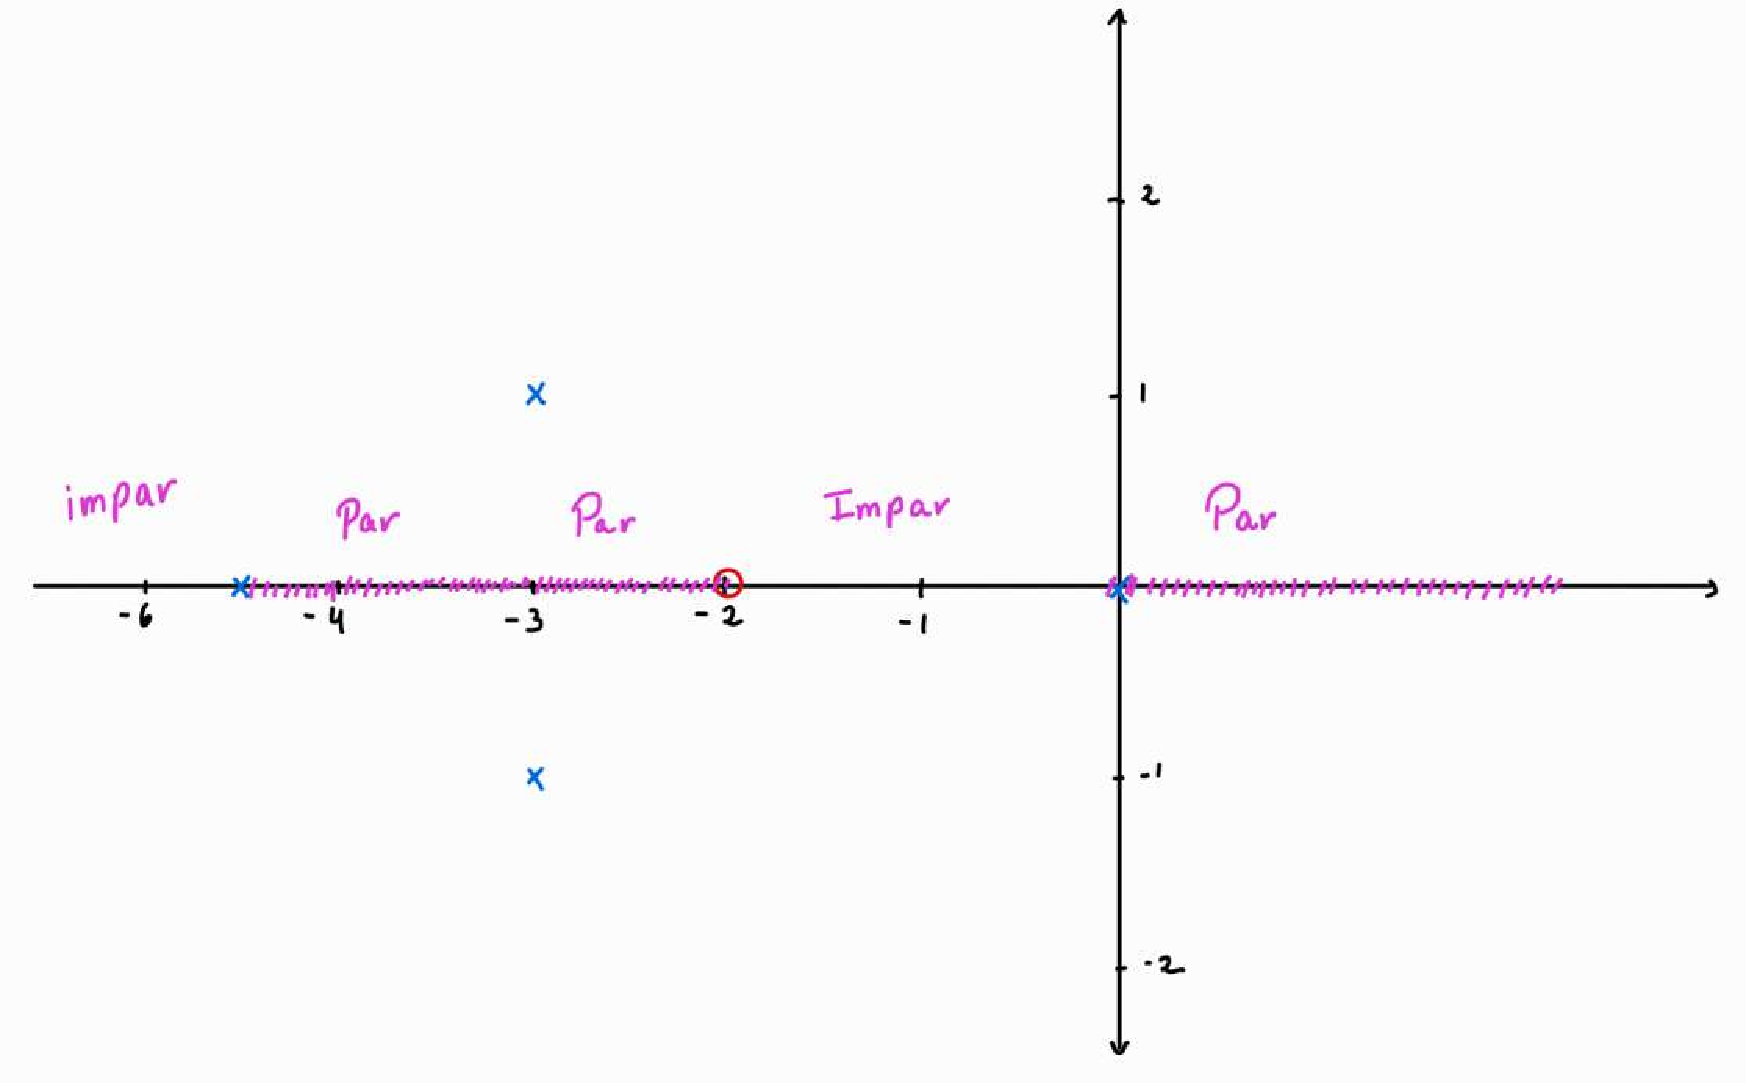
\includegraphics[width=0.7\textwidth]{Auxiliar_2_5}
  \caption{Sistema a analizar.}
\end{figure}
%-----------------------------------------
\begin{solution}
  \subsection*{Resolución 3.1}
Del diagrama de bloques, la salida es la diferencia entre las dos ramas filtradas con $h[n]=a^n u[n]$ y un retardo de 2 muestras en la rama inferior:
\begin{align}
  y[n] &= (x*h)[n] - (x*h)[n-2].
\end{align}
Sea $F[n]=(x*h)[n]$. Para explotar que $x$ es combinación de escalones, resulta útil la \emph{respuesta al escalón} de $h$, que definimos como
\begin{align}
  S[n] = (u*h)[n] = \sum_{k\in\mathbb{Z}} u[k] \, a^{\,n-k} \, u[n-k].
\end{align}
Como $u(k)$ y $u(n-k)$ restringen la sumatoria a $0\le k\le n$, para $n\ge 0$ tenemos
\begin{align}
  S[n] = \sum_{k=0}^{n} a^{\,n-k}
       = a^{\,n} \sum_{k=0}^{n} \left(\frac{1}{a}\right)^{\!k} \quad (a\ne 0) \\
       &= a^{\,n} \, \frac{1-\left(\frac{1}{a}\right)^{\!n+1}}{1-\frac{1}{a}}\,u[n]
       = \frac{1-a^{\,n+1}}{1-a}\,u[n],\qquad (a\ne 1).
\end{align}
Para esto utilizamos la identidad geométrica de la sumatoria con $r=1/a$:
\begin{align}
  \sum_{k=0}^n r^k = \frac{1-r^{n+1}}{1-r}, \quad r \neq 1.
\end{align}
Recordemos que la entrada es un pulso rectangular de longitud 15:
\begin{align}
  x[n] = u[n+5] - u[n-10]
\end{align}
Por linealidad,
\begin{align}
  F[n] = (x*h)[n] = (u[n+5]*h)[n] - (u[n-10]*h)[n] = S[n+5] - S[n-10].
\end{align}
Finalmente,
\begin{align}
  y[n] = F[n] - F[n-2] = [S[n+5] - S[n-10]] - [S[n+3] - S[n-12]].
\end{align}
Sustituyendo $S(\cdot)$ y simplificando, obtenemos la expresión cerrada
\begin{align}
  y[n]
  &= \frac{a^{\,n+6}-1}{a-1} \, u[n+5]
   - \frac{a^{\,n-9}-1}{a-1} \, u[n-10] \\
  &\quad - \frac{a^{\,n+4}-1}{a-1} \, u[n+3]
   + \frac{a^{\,n-11}-1}{a-1} \, u[n-12].
\end{align}
Con ello queda determinada la solución. Para $-1<a<1$, las colas exponenciales decaen fuera del soporte del pulso de entrada.
\end{solution}
%%%%%%%%%%%%%%%%%%%%%%%%%%%

\question Demuestre que, si un sistema cumple
\[ y[n]=T(x[n])=x[n]*h[n]=\sum_{k\in\mathbb{Z}} x[k] \, h[n-k], \]
entonces, con \(h[n]\) la respuesta al impulso del sistema, necesariamente el sistema es lineal e invariante en el tiempo (LTI).
%------------------------------------


\begin{solution}
\subsection*{Resolución 4.1}
  Tomando como Hipotesis que existe una secuencia fija $h[n]$ tal que, para toda $x[n]$,
  \begin{equation}
y[n] = T(x[n])= (x*h)[n] =\sum_{k\in\mathbb Z} x[k]\,h[n-k].
\end{equation}
(En particular, $h[n]=T(\delta[n])$ es la respuesta al impulso.)

\paragraph{(i) Linealidad.}
Para $x_1,x_2$ y $\alpha,\beta\in\mathbb C$:
\begin{align}
T(\alpha x_1+\beta x_2)[n]
&= \sum_{k} \big(\alpha x_1(k)+\beta x_2(k)\big)\,h[n-k] \nonumber\\
&\Rightarrow \alpha \sum_{k} x_1(k)\,h[n-k]+\beta \sum_{k} x_2(k)\,h[n-k] \nonumber\\
&= \alpha\,T(x_1[n])+\beta\,T(x_2[n]).
\end{align}
Luego, $T$ es \textbf{lineal}.

\paragraph{(ii) Invariancia en el tiempo.}
Recordando el operador de traslación $T_k$ dado por $T_k(x[n])=x[n-k]$. Entonces
\begin{align}
T\big(T_k(x[n])\big)
&= \sum_{r \in \mathbb{Z}} x(r-k)\,h(n-r) \nonumber\\
&\overset{m=r-k}{=} \sum_{m} x(m)\,h\big(n-(m+k)\big) \nonumber\\
&= \sum_{m} x(m)\,h\big((n-k)-m\big)
 = T(x[n-k]) = T_k(T(x[n])).
\end{align}
Por tanto, $T\big(T_k(x[n])\big)=T_k(T(x[n]))$ para todo $k\in\mathbb Z$; por lo tanto, $T$ es \textbf{invariante en el tiempo}.

\end{solution}
%------------------------------------------

\question Tres sistemas con respuestas al impulso \(h_1[n]=\delta[n]-\delta[n-1]\), \(h_2[n]=h[n]\) y \(h_3[n]=u[n]\) se conectan en cascada.
\begin{enumerate}
  \item ¿Cuál es la respuesta al impulso total \(h_c[n]\) del sistema en su conjunto?
  \item ¿El orden de conexión afecta al sistema en su conjunto? Justifique.
\end{enumerate}
%--------------------
\begin{solution}
  \subsection*{Resolución 5.1}
  Se busca hallar la \emph{respuesta al impulso total} de la cascada. Las respuestas dadas son
  \[ h_1[n]=\delta[n]-\delta[n-1],\qquad h_2[n]=h[n],\qquad h_3[n]=u[n]. \]
  Para sistemas LTI en cascada, la respuesta equivalente es la \emph{convolución} de las individuales. Usaremos la definición
  \[
    (f*g)[n]\;\triangleq\;\sum_{k\in\mathbb{Z}} f[k] \, g[n-k].
  \]
  Por asociatividad, escribimos
  \begin{align}
    h_c[n] 
    &= \big(h_1*h_2*h_3\big)[n]
     = h_2 * \big(h_1*h_3\big)[n].
  \end{align}
  Cálculo de $(h_1*h_3)[n]$ usando la suma de convolución:
  \begin{align}
    (h_1*h_3)[n]
      &= \sum_{k\in\mathbb{Z}} h_1[k] \, u[n-k]
       = \sum_{k\in\mathbb{Z}} \big(\delta[k]-\delta[k-1]\big) \, u[n-k]\\
      &= \underbrace{\sum_{k} \delta[k] \, u[n-k]}_{=\,u[n]}
       \, - \, \underbrace{\sum_{k} \delta[k-1] \, u[n-k]}_{=\,u[n-1]} \\
      &= u[n]-u[n-1].
  \end{align}
  Notemos que $u[n]-u[n-1]=\delta[n]$ (la diferencia de dos funciones escalón unitario es la función impulso); en consecuencia,
\begin{align}
  h_{c}[n] = h_2 * \delta[n] = h_2[n] = h[n].
\end{align}
  \[
    \boxed{\,h_c[n]=h[n].\,}
  \]


  \subsection*{Resolución 5.2}
Para sistemas LTI, la convolución es \emph{conmutativa} y \emph{asociativa}, por lo que
  \[
    h_1*h_2*h_3 = h_{\sigma(1)}*h_{\sigma(2)}*h_{\sigma(3)}\quad \text{para cualquier permutación }\sigma.
  \]
  Además, como ya vimos que $h_1*h_3=\delta$, agrupando por asociatividad se obtiene, en cualquier orden,
  \[
    h_c(n) = h_2*\delta(n) = h_2(n) = h(n).
  \]
  Por lo tanto, \textbf{el orden no afecta} al sistema en su conjunto; la cascada siempre es equivalente a un filtro con respuesta $h(n)$.
\end{solution}

%------------------

\question Considere el sistema a tiempo discreto de orden $N$ caracterizado por la siguiente ecuación de diferencia con parámetros constantes $b_1,\ldots,b_N$ y $a_0,\ldots,a_M$:
\begin{equation}
\label{eq:edo}
 y[n] = b_1 \, y[n-1]+\cdots+b_N \, y[n-N] + a_0 \, x[n]+\cdots+a_M \, x[n-M],
\end{equation}
para todo $n\in\mathbb{Z}$. Supondremos \emph{coeficientes constantes en el tiempo} y señales definidas en $\mathbb Z$.

\begin{parts}
  \part Verifique que el sistema determinado en la Ec.~\eqref{eq:edo} es lineal.
  \part Verifique que el sistema determinado en la Ec.~\eqref{eq:edo} es invariante en el tiempo (TI).
  \part Considere la versión con condiciones iniciales del sistema en \eqref{eq:edo}: $y[n]$ se determina para $n\ge 0$ donde la entrada es $\big(x[n]\big)_{n\ge 0}$ (asumiendo valores nulos en tiempos negativos) y el vector de estado (condiciones iniciales de \eqref{eq:edo}) es $y_1=y[-1],\ldots,y_N=y[-N]$. Verifique que la solución frente a la entrada $\big(x[n]\big)_{n\ge 0}$ y las condiciones iniciales $(y_1,\ldots,y_N)$ se puede escribir como
  \begin{equation}
    \big(y[n]\big)_{n\ge 0} = \big(y_{SO}[n]\big)_{n\ge 0} + \big(y_{IO}[n]\big)_{n\ge 0},
  \end{equation}
  donde $\big(y_{SO}[n]\big)_{n\ge 0}$ denota la \emph{respuesta de estado cero} y $\big(y_{IO}[n]\big)_{n\ge 0}$ denota la \emph{respuesta de entrada cero}.
\end{parts}

%---
\begin{solution}

\subsection*{Resolución 6.1}
Dado el operador $T$ por la relación entrada-salida
\[
  T(x[n]) = y[n] \quad \text{tal que} \quad
  y[n]=\sum_{k=1}^{N} b_k\,y[n-k]+\sum_{m=0}^{M} a_m\,x[n-m],\qquad n\in\mathbb Z.
\]
 Sean $x_1\mapsto y_1=T(x_1)$ y $x_2\mapsto y_2=T(x_2)$. Definamos
\( z[n] = \alpha y_1[n] + \beta y_2[n] \). Entonces, utilizando únicamente propiedades algebraicas,
\begin{align}
  z[n]
   &= \alpha y_1[n] + \beta y_2[n] \\
   &= \alpha\Big(\sum_{k=1}^{N} b_k\,y_1[n-k] + \sum_{m=0}^{M} a_m\,x_1[n-m]\Big)
    \, +\, \beta\Big(\sum_{k=1}^{N} b_k\,y_2[n-k] + \sum_{m=0}^{M} a_m\,x_2[n-m]\Big) \\
   &= \sum_{k=1}^{N} b_k\,[\alpha y_1[n-k]+\beta y_2[n-k]]
      + \sum_{m=0}^{M} a_m\,[\alpha x_1[n-m]+\beta x_2[n-m]].
\end{align}
Es decir, $z$ satisface la misma ecuación con la entrada $\alpha x_1+\beta x_2$. Por lo tanto,
\[
  T(\alpha x_1+\beta x_2)[n] = z[n] = \alpha T(x_1)[n] + \beta T(x_2)[n].
\]
\[\boxed{\text{El sistema es lineal.}}\]

\subsection*{Resolución 6.2}
Sea $T_k$ el operador de desplazamiento temporal: $T_k(x[n])=x[n-k]$. Debe cumplirse que
\begin{equation}
  T_k\big(T(x[n])\big) \,=\, T\big(T_k(x[n])\big).
\end{equation}
\noindent
Primera rama:
\begin{align}
  T(x[n]) &= \sum_{i=1}^{N} b_i\,y[n-i] + \sum_{m=0}^{M} a_m\,x[n-m], \\
  T_k\!\left(T(x[n])\right) &= \sum_{i=1}^{N} b_i\,y[(n-k)-i] + \sum_{m=0}^{M} a_m\,x[(n-k)-m].
\end{align}
Por otro lado (segunda rama):
\begin{align}
  T_k(x[n]) &= x[n-k], \\
  T\big(T_k(x[n])\big) &= \sum_{i=1}^{N} b_i\,y[n-k-i] + \sum_{m=0}^{M} a_m\,x[n-k-m].
\end{align}
Como
\[
  T_k\big(T(x[n])\big) = T\big(T_k(x[n])\big),
\]
el sistema es \textbf{invariante en el tiempo}.

\subsection*{Resolución 6.3}
Consideremos el caso causal $n\ge 0$, con $x[n]=0$ para $n<0$ y condiciones iniciales
$y[-1]=y_1,\dots,y[-N]=y_N$. Verificaremos que la solución asociada a la entrada $\big(x[n]\big)_{n\ge 0}$ y a dichas condiciones iniciales puede escribirse como
\begin{equation*}
  y[n] \;=\; y_{SO}[n]+y_{IO}[n], \qquad n\ge 0,
\end{equation*}
donde:
\begin{itemize}
  \item $y_{SO}$: solución con \emph{condiciones iniciales nulas} y entrada $x$.
  \item $y_{IO}$: solución con \emph{entrada nula} y condiciones iniciales dadas.
\end{itemize}
En términos de la ecuación de diferencia, ambas se describen explícitamente por
\begin{align}
  y_{SO}[n] &= \sum_{k=1}^{N} b_k\,y_{SO}[n-k] + \sum_{m=0}^{M} a_m\,x[n-m],
  & y_{SO}[-k]&=0,\quad k=1,\dots,N, \\
  y_{IO}[n] &= \sum_{k=1}^{N} b_k\,y_{IO}[n-k]
  + \underbrace{\sum_{m=0}^{M} a_m\,x[n-m]}_{=\,0\ \text{(entrada nula)}},
  & y_{IO}[-k]&=y_k,\quad k=1,\dots,N.\quad (x[n]\equiv 0)
\end{align}
Si definimos $y[n]\triangleq y_{SO}[n]+y_{IO}[n]$, entonces,
\begin{align}
  y[n]
  &= y_{SO}[n]+y_{IO}[n] \\
  &= \Big(\sum_{k=1}^{N} b_k\,y_{SO}[n-k] + \sum_{m=0}^{M} a_m\,x[n-m]\Big)
   + \Big(\sum_{k=1}^{N} b_k\,y_{IO}[n-k] + 0\Big) \\
  &= \sum_{k=1}^{N} b_k\,\big(y_{SO}[n-k]+y_{IO}[n-k]\big)
     + \sum_{m=0}^{M} a_m\,x[n-m] \\
  &= \sum_{k=1}^{N} b_k\,y[n-k] + \sum_{m=0}^{M} a_m\,x[n-m],
\end{align}
es decir, $y$ satisface la misma ecuación de diferencia con la entrada $x$. Además, para $k=1,\dots,N$,
\begin{align}
  y[-k] = y_{SO}[-k]+y_{IO}[-k] = 0 + y_k = y_k,
\end{align}
por lo que $y$ cumple las \emph{mismas} condiciones iniciales. Por unicidad de soluciones de una recurrencia lineal de orden $N$,
\[
  \boxed{\,y = y_{SO}+y_{IO}.\,}
\]

\subsection*{Resolución 6.4 }
Sea $T_0: x\mapsto y_{SO}$ (estado cero).
\begin{itemize}
  \item \textbf{Linealidad:}
  si $x_1\mapsto y_{SO,1}$ y $x_2\mapsto y_{SO,2}$, entonces
  \begin{equation}
    T_0[\alpha x_1+\beta x_2]=\alpha y_{SO,1}+\beta y_{SO,2}.
  \end{equation}
  Tenemos que esto se puede ver en lo siguiente:
  \begin{align}
    T_0[\alpha x_1+\beta x_2][n]
      &= \sum_{k=1}^{N} b_k\,(\alpha y_{SO,1}[n-k]+\beta y_{SO,2}[n-k])
         + \sum_{m=0}^{M} a_m\,(\alpha x_1[n-m]+\beta x_2[n-m]) \\
      &= \alpha T_0(x_1[n]) + \beta T_0(x_2[n]).
  \end{align}
  \item \textbf{Invariancia temporal:}
  definamos el operador de desplazamiento $T_k$ por $T_k(x[n])=x[n-k]$,
  \begin{equation}
    T_0\big(T_k(x[n])\big)= T_k\big(T_0(x[n])\big).
  \end{equation}
  Luego, tenemos que:
  \begin{align}
    T_0(T_k x[n])
      &= \sum_{i=1}^{N} b_i\,y_{SO}[n-k-i] + \sum_{m=0}^{M} a_m\,x[n-k-m] \\
      &= T_k\,T_0(x[n]).
  \end{align}
\end{itemize}
Luego, \(\boxed{T_0 \text{ es LTI.}}\). Si se trabaja en la ventana causal $n\ge 0$, la TI se mantiene para corrimientos $k\ge 0$ que preservan el “pasado nulo”. Corrimientos que cruzan el borde ($k<0$) introducen efectos de borde y rompen la TI en esa ventana.
\end{solution}




\end{questions}
\end{document}